\documentclass{article}
\usepackage[utf8]{inputenc}
\usepackage{graphics}
\usepackage{graphicx}

\author{Ondrej Podhorsky\\[2pt]
	{\small Slovenská technická univerzita v Bratislave}\\
	{\small Fakulta informatiky a informačných technológií}\\
	{\small \texttt{xpodhorsky@stuba.sk}}
	}

\date{\small 6. november 2022}

\begin{document}

\maketitle

\begin{abstract}

Obsahom tohto článku je čitateľovi priblížiť aplikáciu umelej inteligencie vo video hernom priemysle, dejiny a minulosť uplatnenia. Umelá inteligencia ako má tento článok ukázať, má za ciel riešenie komplexných problémov pomocou stroja v hrách, čiže napríklad v oblastiach samotného vývoja, fungovania a hrateľnosti . Zároveň takáto aplikácia takýchto algoritmov má v súčasnosti určité limitácie na, ktoré bude snaha poukázať a prípadne nájsť použitelné a vhodné možnosti riešenia.

\end{abstract}

\clearpage

\section{Úvod}

Cieľom tohto článku je priblížiť použitie a možnosti použitia umelej inteligencie v video hernom priemysle, ktorý sa v súčasnosti dostáva do popredia v zábavnom priemysle. V roku 2022 by mal podľa očakávaní mať výnos 225 biliónov dolárov \cite{TeodoraDobrilovat}, čo by ho radilo napríklad pred hudobný alebo filmový priemysel. Dlhodobo sa snažili najpoprednejšie štúdia vyvíjať hry s dôrazom  na grafickú realistickosť. No v podstate tento ciel už bol dosiahnutý a preto sa snažia implementovať iné technológie do svojich hier, ktorými by sa dal obohatiť video herný zážitok, zjednodušiť ich vývin či testovanie hier. Prvá časť bude obsahovať informácie o disciplíne, ktorú použitie umelej iteligencie definovalo. V ďalších častiach sa bude písať o aspektoch hry, ako je napríklad tvorba a fungovanie nehráčských postáv a jej limitáciám, vylepšením tvorby herného zážitku implentovaním umelej inteligencie do herných mechaník a generovaním obashu pre zjednodušenie práce herných vývojárov.

\begin{figure}[ht]{1. Aplikácia umelej inteligencie v hrách\cite{inproceedings}}
\centering
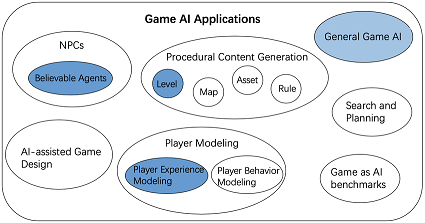
\includegraphics[width=103mm]{Game-AI-Applications.png}
\end{figure}

\begin{figure}[ht]
\centering
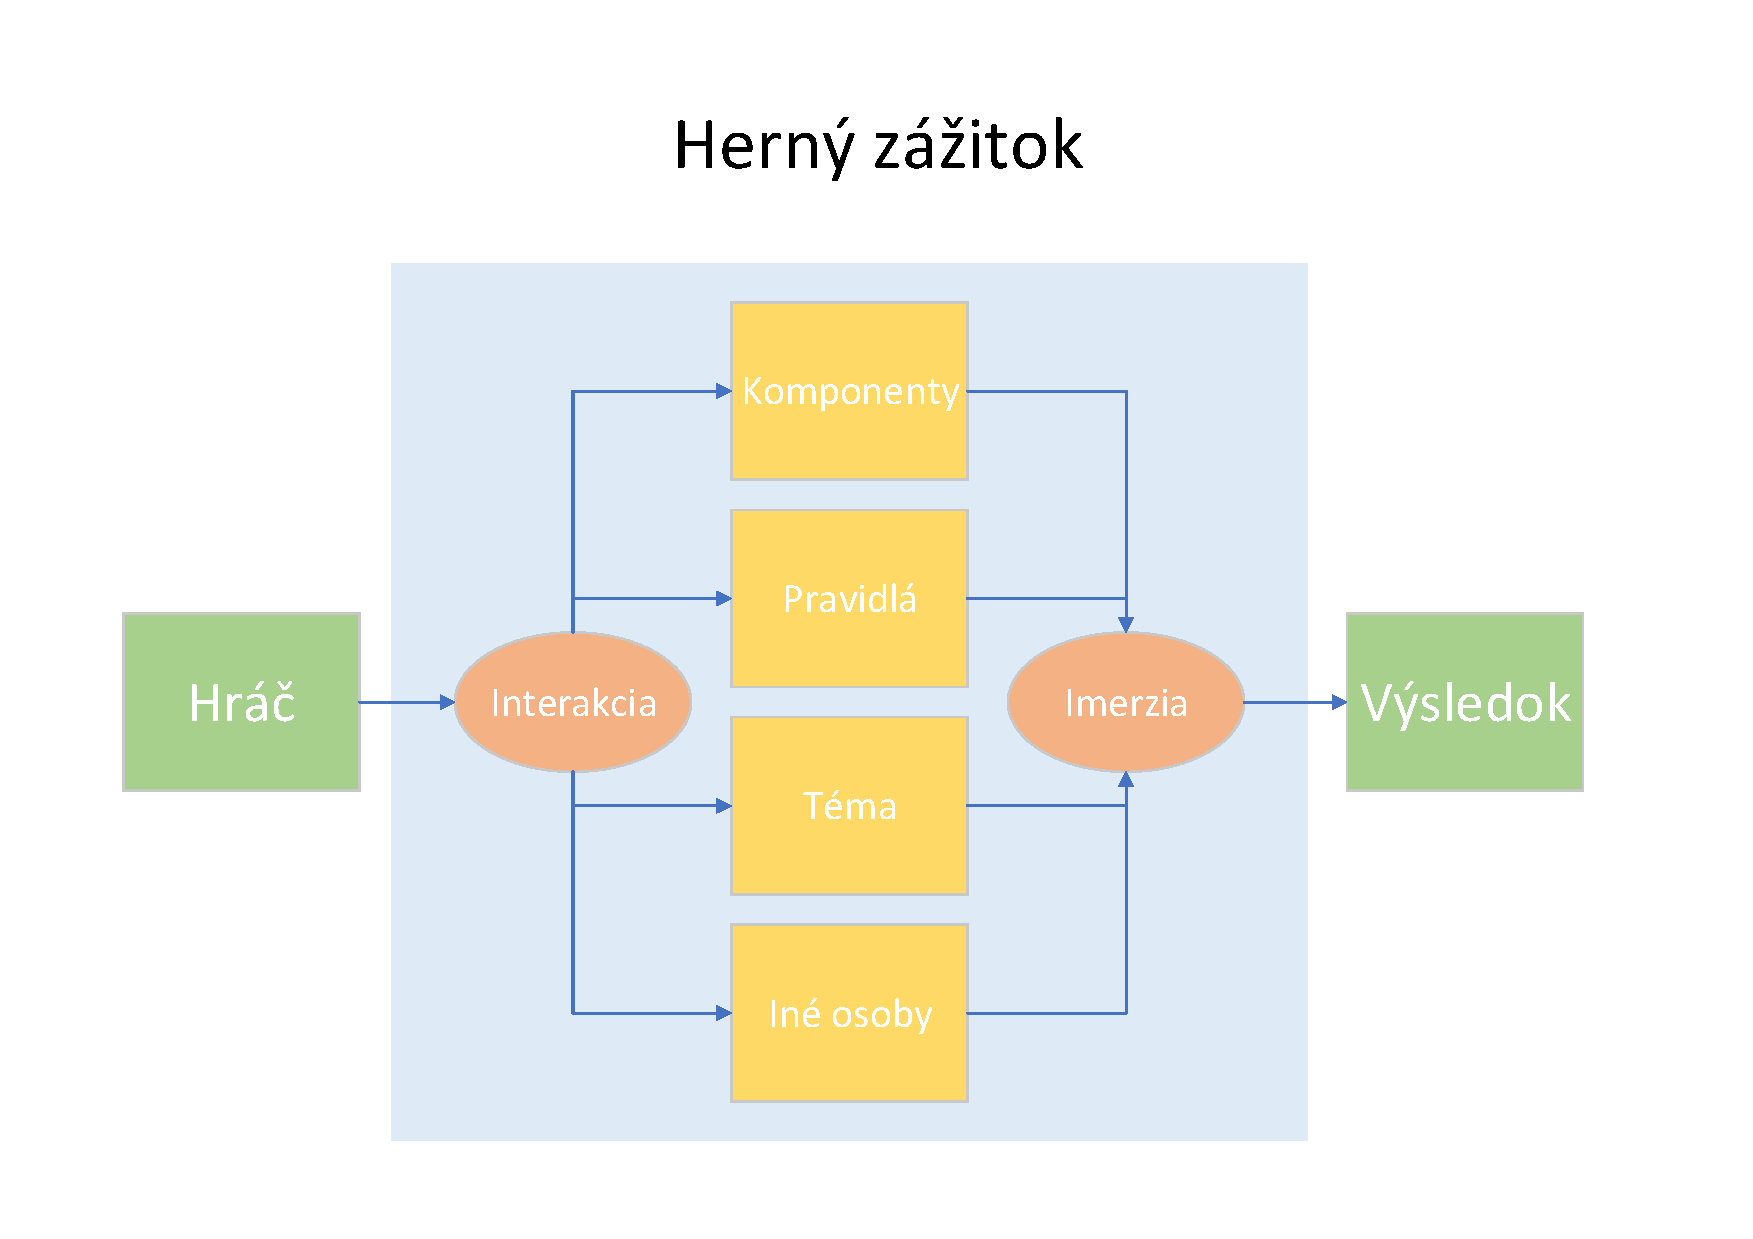
\includegraphics[width=83mm]{Herný zážitok diagram.pdf}
\end{figure}

\clearpage

\section{Hry ako testovacie prostredie}
\subsection{Klasické hry}

Hry boli odzačiatku vzniku prvých algoritmov pre vedcov ihrysko, kde mohli testovať najnovšie technológie. V roku 1951 Christopher Strachey  napísal program pre dámu a Dietrich Prinz pre šach \cite{Copeland}. Klasické doskové hry boli ideálne pre testovanie s pevnými pravidlami no zároveň komplexné. Cielom bola snaha poraziť človeka v týchto hrách. Veľkým milníkom sa stal šachový zápas medzi veľmajstrom Kasparovom a IBM Deep Blue v roku 1997, ktorý Deep Blue na koniec vyhral 4-2. Alebo nedávne výťaztvo Google Deeps mind Alpha go v hre go nad svetovým šampión Lee Sedolom\cite{Reuters}. Go je najkomplexnejšia dosková z klasických abstraktných hier a preto sa v súčastnosti prechádza na komplikovanejšie tituli.

\begin{table}[ht]
\caption {2. Úspechy umelej inteligencie proti ľuďom} \label{tab:title} 
\resizebox{\textwidth}{!}{\begin{tabular}{|l|l|l|l|l|}
\centering
\hline
Hra                  & Súper                                           & Rok  & Umelá inteligencia & Firma, inštitúcia            \\ \hline
Dáma                 & Marion Tinsley                                  & 1994 & Chinook                     & University of Alberta        \\ \hline
Šach                 & Garry Kasparov                                  & 1997 & Deep Blue                   & IBM                          \\ \hline
GO                   & Lee Sedol                                       & 2016 & AlphaGo                     & Google DeepMind              \\ \hline
Texas hold'em(poker) & J. Les, D. Kim, J. Chuo, D. McAulay & 2017 & Libratus                    & Carnegie Mellon University's \\ \hline
\end{tabular}}
\end{table}

\subsection{Počítačové hry}
Video hry majú rôzne žánre, niektoré v hodné pre výskum a niektoré až tak moc nie. Strielačky a bojové hry môžme hneď na začiatku vylúčiť z dôvodu že počítač má samozrejme obrovskú výhodu oproti ľuďom kôli nadľudskému reakčnému času a schopnosti strelby. Ťahové strategické hry sú tiež len v podstate komlikovanejší šach s väčším množstvom možností a s menej priamočiarimy cielmy. No sú tu aj hry odohrávajúce sa v reálnom čase, ktoré predstavujú pre vedcov väčšiu výzvu. No v roku 2019 sa podarilo Alpha Star od Deep mindu poraziť viacerých profesionálov v hre Star Craft II a OpenAI Five ešportový tím svetových šampiónov v hre Dota II. Na rozdiel od Alpha staru sa musel OpenAI Five potýkať s nutnosťou riešenia kooperácie keďže Dota II je kooperatívna tímová hra.

\subsection{Neperfektné hry}

Jednou s takychto hier je napríklad kartová hra texas hold'em, ľudovo nazývaná poker, ktorá sa radí medzi neperfektné vďaka tomu že, hráč si nemôže byť stopercentne istý aký bude mať hra výsledok a pracuje tak iba s pravdepodobnosťami, taktiež hráči nemajú rovnaké informácia. Pre takéto hry je obtiažne vymyslieť algoritmy, kôli rôznorodým premenným, ktoré do nich vstupujú. Ako prvej umelej inteligencie, ktorá prekonala tieto prekážky a pokorila štyroch vrcholových hráčov v maratóne pokru v hre o 1,7 milióna dolárov v roku 2017, kde hráči hrali v dvojiciach proti sebe, sa stala Libratus vytvorená univerzitou Carnegieho–Mellonových z Pensylvánie\cite{Reuters}. Na tento úspech tím z spomínanej univerzity nadviazal a v roku 2019, keď porazili v hre viacerých hráčov šesť profesionálov\cite{Nature}. 

\subsection{Sociálne hry}

Hry majú aj svoju socialnu stránku, teda v hre sa nachádzajú prvky diplomacie, obchodu, kooperácie a je nutné mať pri nich schopnosť jasne sa dorozumievať s ostatnými hráčmi. Napríklad už spomínaná kartová hra poker má aj sociálny prvok a to je takzvané blufovanie, kde hráč svojou hrou chce presvedčiť súpera, že má lepšie karty na ruke než v skutočostni vlastní. Bez schopnosti blufovať a rozpoznať či niekto blufuje by nikto nevedel dosiahnuť špičkovej úrovne v pokru, no Libratus to dokáže s nesmiernou presnosťou. Analizuje predošlé hry súpera, súčastnú sytuáciu a primerane sa rozhodne. Ďalšou z pár takýchto sociálnych hier, ktorú umelá inteligenicia dokázala "poraziť" je Diplomacia\cite{doi:10.1126/science.ade9097}. Ako jej meno napovedá, hnacím motorom je diplomacia. A tu prichádza problém lebo posilnené učenie sa tu nedá použiť. Keď hrá počítač len proti sebe, tak dosiahne nadludských výkonov ale keď rovnaký algoritmus dosadíme do prostredia s viacerímy hráčmi, kde je nutnosť kooperácie tak je prakticky nepoužitelný. Cicero, program ktorý tieto problémy vyriešil, od firmy meta. Na diagrame je prehlade ukázané ako funguje.

\begin{figure}{2. Architektúra Cicera\cite{doi:10.1126/science.ade9097}}
\centering
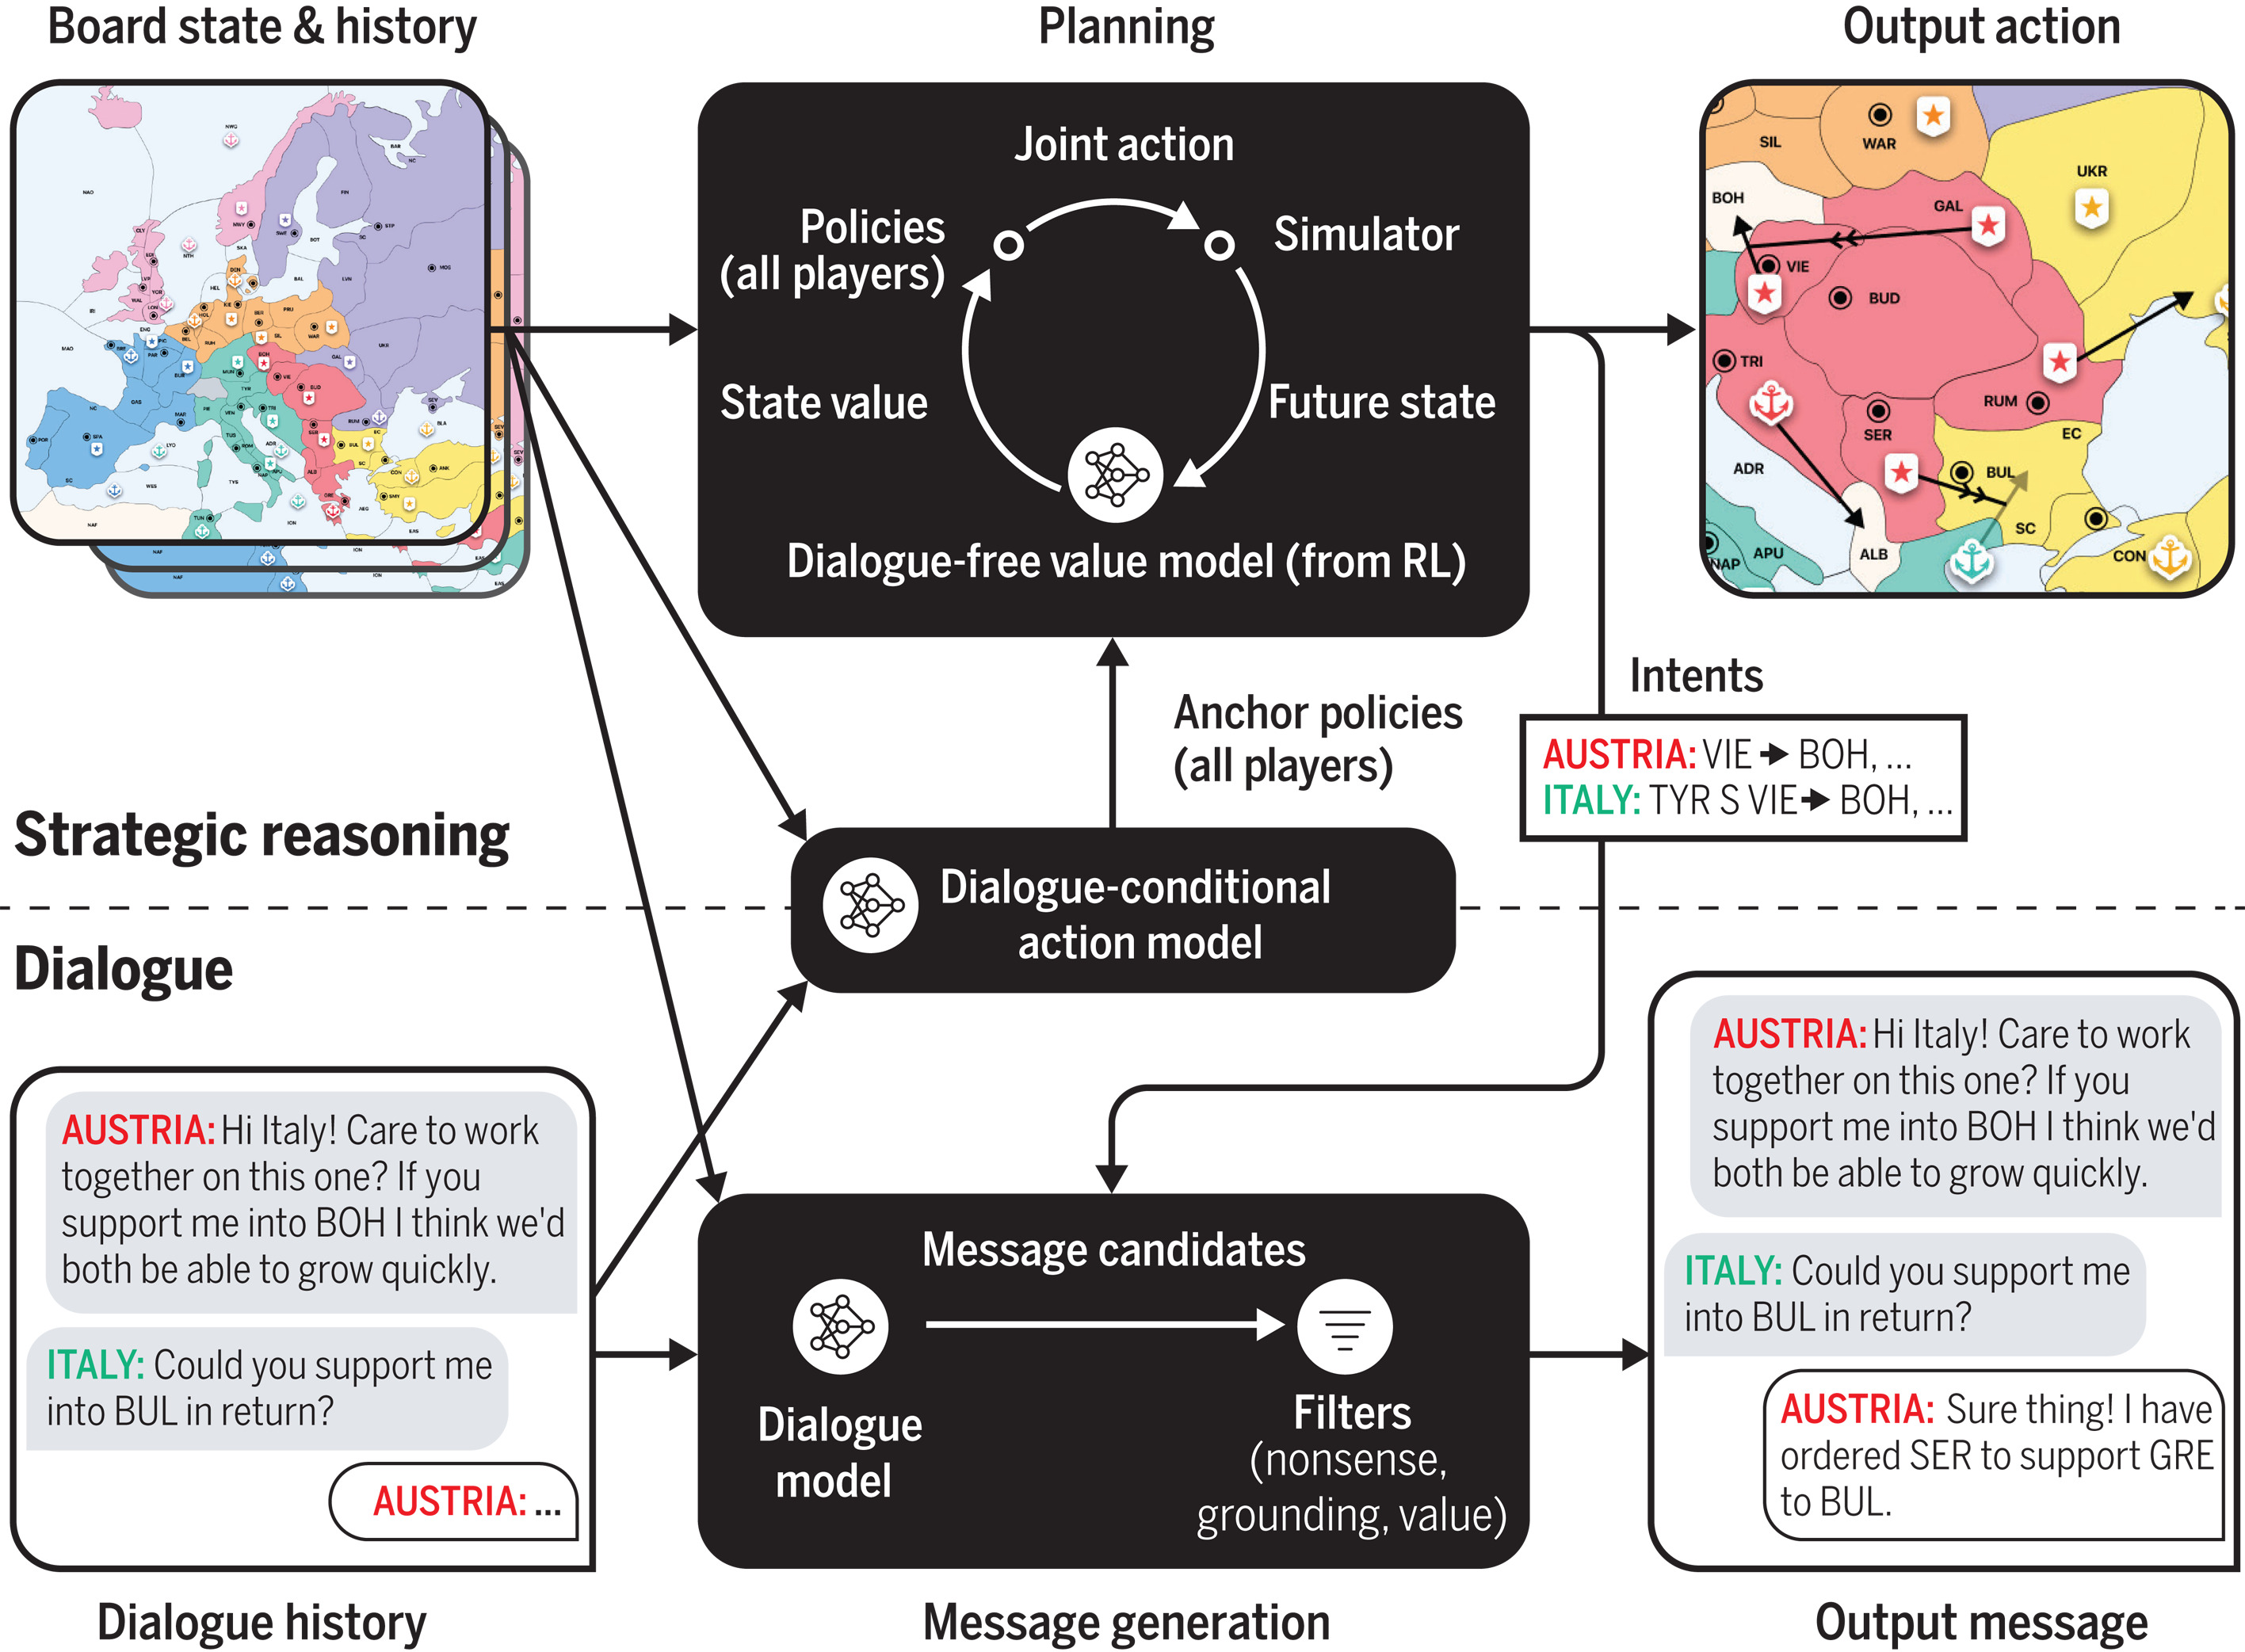
\includegraphics[width=103mm]{science.ade9097-f1.jpg}
\end{figure}
Cicero predpovedá pravdepodobnosť ťahov pre každého hráča podľa stavu hry a histórie dialógu, pričom to použije ako východiskový bod pre plánovací algoritmus využívajúci trénované  modely. Výstupom plánovania je akcia pre agenta, ako aj predstava o akciách ostatných hráčov, ktoré sa neskôr používajú na výber zámerov pre model dialógu, ktorým sa má podmieniť. Vygenerovaní kandidáti na správu podstúpia niekoľko krokov filtrovania pred odoslaním konečnej správy.

\subsection{Potenciál}

Na vzdory niektorých odborníkov, ktorý tvrdia že existujú iné alternatívy vyskumného prostredia, pre mnohých iných sú hry hlavne kultúrnov vynikajúce kôli ich roli v spoločnosti. Nie vždy sú vedci schopný naplniť štadióny a titulky časopisov svojimy objavmy. No napriek tomu súčasné algoritmy sa ťažko adaptujú a iné prostredie a na riešenie reálnych problémov. Sú veľmi krehké a príliš špecializované napríklad Deepmind od Googlu iba pri najmenšej zmene Star Craft II jeho výkon výrazne degraduje. Aj tak sa nájdu aj výnimky. 
\section{Nehráčske postavy}

Nehráčske postavy sú neodmysliteľnou časťou hier od nepamäti. Sú to prevažne charaktery, ktoré ovláda počítač po prípade hráč. No v súčasnosti je to časť hry, ktorá sa často prehliada a priorita sa hlavne prikladá na grafickú stránku hier. Umelá inteligencia má potenciál tento problém vyriešiť. Momentálne sa prevažne používajú primitívne postupy vytvorené ešte v 90tich rokoch, ktoré sú napríklad pathfinding,finite state machines alebo komplexnejšie ako je napríklad Monte Carlo Tree Search\cite{nickstatt}. Vývojári v posledných dekádach len zväčšujú merítko v akom sú tieto koncepty využívané.

\subsection{Limitácie}

Hlavnými obmedzeniami sú nedostatočné výpočtové prostriedky dostupné pre bežného používateľa. Tak tiež nepredvídateľnosť takýchto charakterov by vytvárala chaos a práve naopak by ešte viac znížila pocit prirodzeného správania a podkopala tak video herný zážitok\cite{phdthesis}.

\section{Generovanie herného obsahu}
Procedurálna tvorba herných asetov, zväčšej časti grafiky ale napríklad aj hudby alebo textu o ktorú sa zaoberá veľa spoločností. Motivácia je hlavne finančného keďže tvorba grafiky nie len pre hry ale aj pre filmy, internetové stránky či v oblasti reklamy má za potrebie armády grafikov. Napríklad pre vytvorenie jednej minúty počítačovo vytvorenej snímky vo filme, stojí priemerne 560,000 dolárov. Aplikovanie umelej inteligencie by razantne zredukovalo výdaje.
\subsection{Grafika}
Programy ktoré dokážu takto vytvárať grafiku sa nazývajú generátory grafiky. Sú to NightCafe, DALLE-E 2, Deep Dream Generator. Tieto programy však nevedia vytvárať dynamickú grafiku len 2D obrázky. Priekopníkom v procedurálnom vytváraní grafiky je spoločnosť Nvidia, ktorá pre zaujímavosť vytvorila pomocou videa vytvárať takmer jedna ku jednej grafiku. 
\section{Záver}
Ako tento článok ukázal, že implentovaním umelej iteligencie do počítačových hier, prinesie zlepšenie v hernom zážitku, pokrok k vytvorenie obecnej umelej inteligencie, zlacní ich tvorbu. Novodobý výskup prináša výsledky každým dňom a preto môžme očakáť napredovanie, ktoré nenasvedčuje nič že by ho vedelo spomaliť.
\section{Reakcia na témy}

Kreatívne písanie.
Najviac ma oslovila téma kreatívneho písania, vďaka neskutočnému prístupu Mgr. Aleksandra Vranićovej, ktorá nás oboznámila s možnosťami plynulejšieho, spontánneho písania aj takých rigoróznych prác ako sú vedecké články či vedecké práce. Aj keď osobne som sa písaniu vždy vyhýbal tak mi táto téma dala veľa. 

Prezentácia: slajdy a prednes
Tematika ohladom prezentácii bola v mojich očiach veľmi prínosná. Sám som mal pocit že mojím prezentáciam vždy niečo chýbalo alebo bolo niečo navyše.Taktiež práca s Latexom bola tiež pútajúca. Z hladiska obsahu som sa dozvedel o určitých otázkach ktoré by mala každá prezentácia zodpovedať a mala by mať určitú štruktúru. 
\bibliography{literatura}
\bibliographystyle{plain}
\end{document}
